\documentclass[a4paper,12pt]{article}
\usepackage{url}
\usepackage{caption}
\usepackage{subcaption}
\usepackage{graphicx}
\usepackage{wrapfig}
\usepackage{xcolor}
\begin{document}

\begin{center}
\begin{Large}


\textbf{Assignment 4}

Web Science CS595

Name: Amara Naas
\end{Large}
\end{center}
\pagebreak

\textbf{Answer to question 1}\par
In the Python program (q1\_2.py)\footnote{File uploaded to github} will  extract all of the links from a selected 100\footnote{Saved in res.txt} pages to other pages. For each URI it will create a text file of all of the outbound links from that page to other URIs including the main URI and save it in the files directory\footnotemark[1].
\par

$\:$
%\enspace

\textbf{Answer to question 2}\par
The same Python program (q1\_2.py)\footnotemark[1] will create a single GraphViz "dot" file called gefiDoc.gv\footnotemark[1] of the resulting graph.\par
%\textcolor{red}{[text]}




\textbf{Answer to question 3}\par
In this question I used Gephi and gefiDoc.gv\footnotemark[1] to visualize the graph as shown in figure 1. Also I find out that the most in-link was twitter.com as shown in figure 2 and the must out-link was finance.detik.com as shown in figure 3.
$\:$
%\enspace

From this figures we can observe that many links have a very high out degree and very few have high in degree. 

Also figure 4 shows graph of the HITS, figure 5 shows PageRank, figure 6 shows avg degree, figure 7 shows network diameter, and figure 8 shows connected components.
$\:$
%\enspace



\pagebreak
\begin{figure}
\center
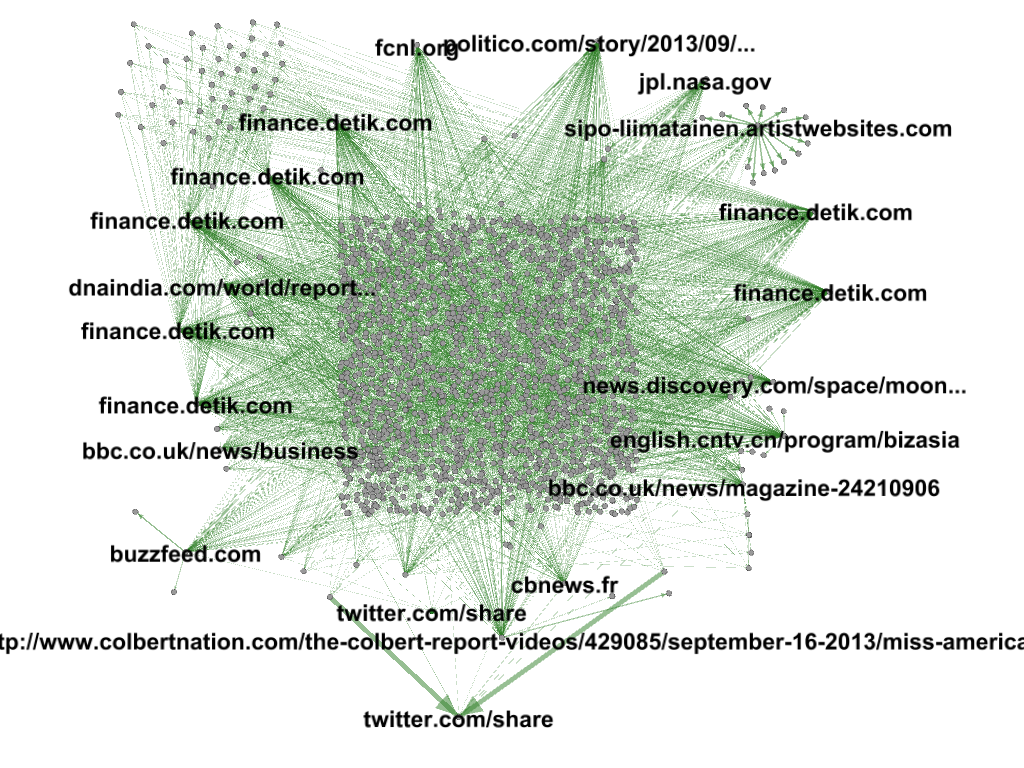
\includegraphics[width=\linewidth]{MainGraph.png} 
\caption{Gephi Graph of "dot" file}
\end{figure}

\begin{figure}
\center
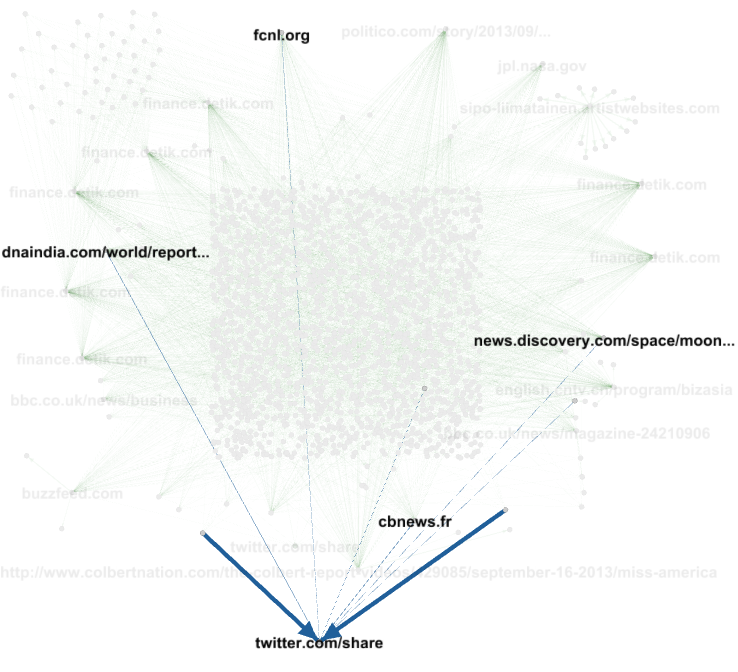
\includegraphics[width=\linewidth]{indegree.png} 
\caption{twitter.com in-degree}
\end{figure}

\begin{figure}
        \centering
        %\begin{subfigure}[b]{0.7\textwidth}
        \begin{subfigure}[a]{0.8\textwidth}
                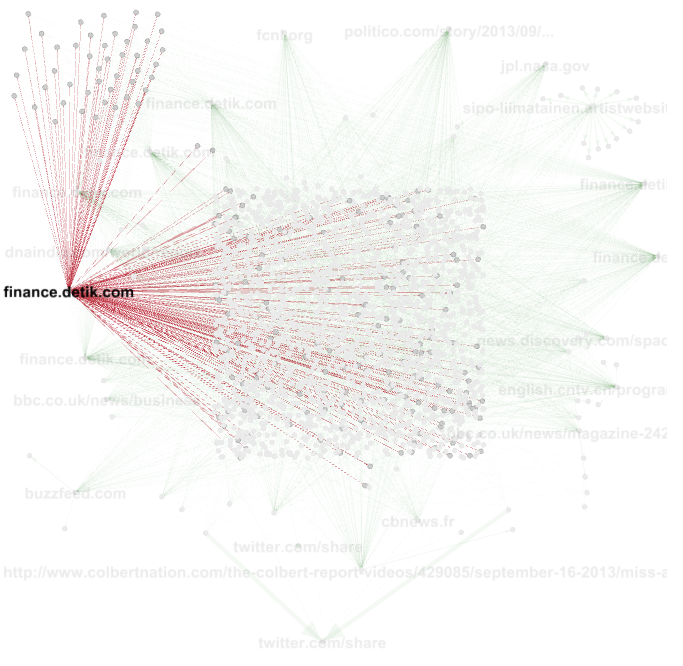
\includegraphics[width=\textwidth]{Outdegree1.png}
                \caption{No link to other finance.detik.com }
               
        \end{subfigure}
        ~ %add desired spacing between images, e. g. ~, \quad, \qquad etc.
          %(or a blank line to force the subfigure onto a new line)
        
        \begin{subfigure}[b]{0.8\textwidth}
                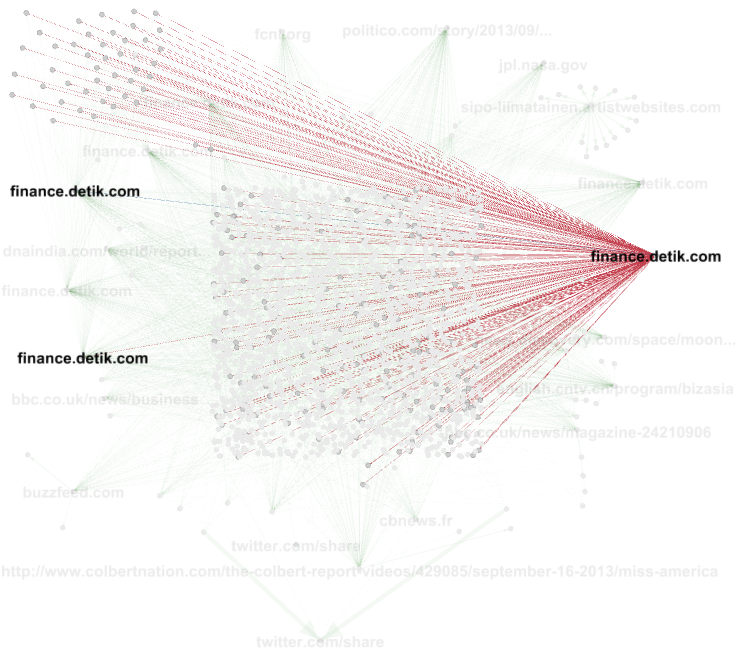
\includegraphics[width=\textwidth]{Outdegree2.png}
                \caption{some links to other finance.detik.com}
                
        \end{subfigure}%
        \caption{finance.detik.com out-degree}
\end{figure}

\begin{figure}
        \centering
        %\begin{subfigure}[b]{0.5\textwidth}
        \begin{subfigure}[a]{1\textwidth}
                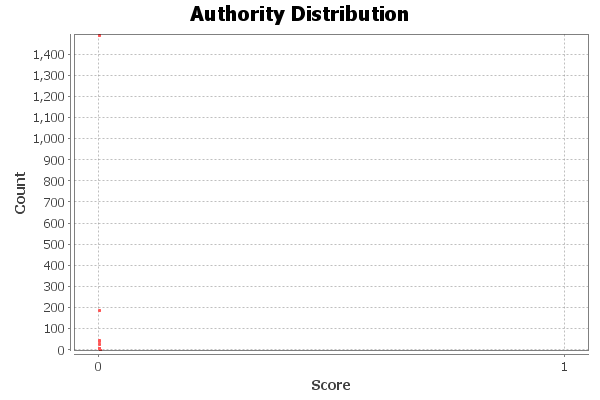
\includegraphics[width=\textwidth]{authorities.png}
                \caption{Authorities Distribution}
               
        \end{subfigure}
        ~ %add desired spacing between images, e. g. ~, \quad, \qquad etc.
          %(or a blank line to force the subfigure onto a new line)
        
        \begin{subfigure}[b]{1\textwidth}
                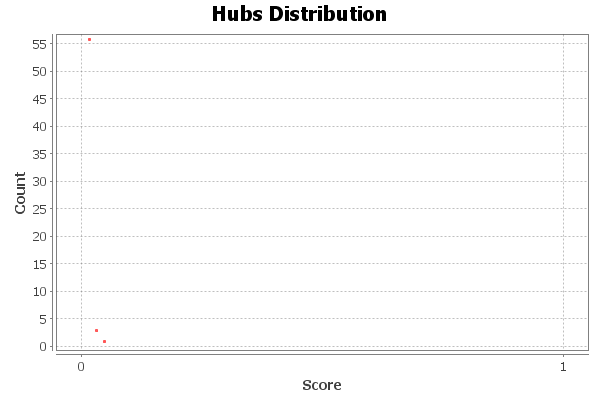
\includegraphics[width=\textwidth]{hubs.png}
                \caption{Hubs Distribution}
                
        \end{subfigure}%
        \caption{HITS}
\end{figure}
\begin{figure}
\center
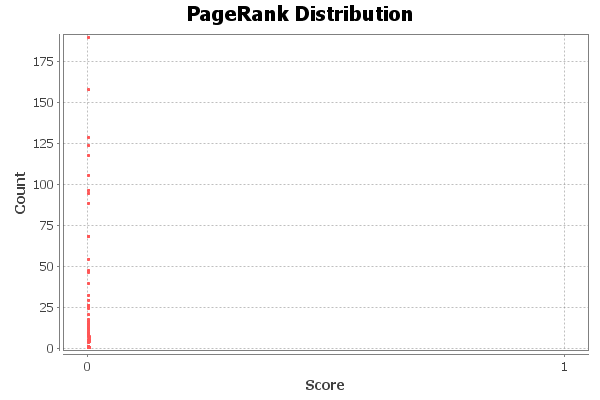
\includegraphics[width=\linewidth]{pageranks.png} 
\caption{PageRank}
\end{figure}

\begin{figure}
        \centering
        \begin{subfigure}[a]{0.675\textwidth}
                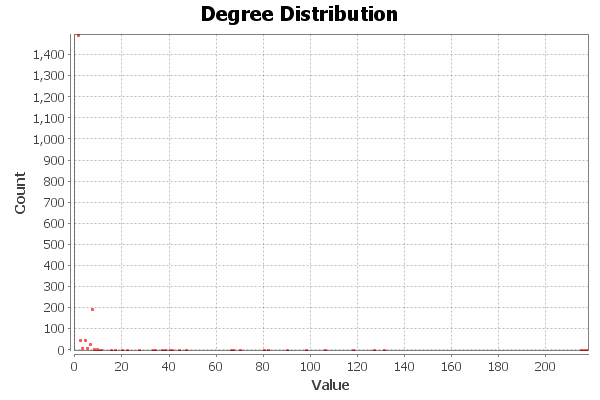
\includegraphics[width=\textwidth]{degree-distribution.png}
                \caption{Degree Distribution}
               
        \end{subfigure}
        ~ %add desired spacing between images, e. g. ~, \quad, \qquad etc.
          %(or a blank line to force the subfigure onto a new line)
        
        \begin{subfigure}[b]{0.675\textwidth}
                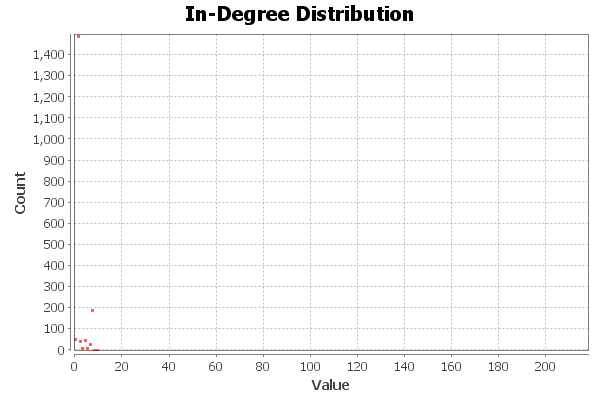
\includegraphics[width=\textwidth]{indegree-distribution.png}
                \caption{In-degree Distribution}
                
        \end{subfigure}%
        
         \begin{subfigure}[c]{0.675\textwidth}
                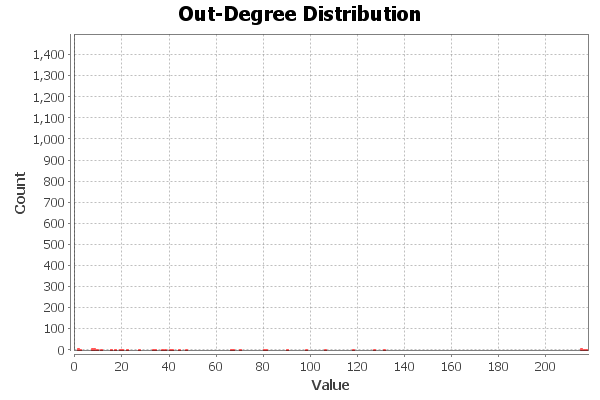
\includegraphics[width=\textwidth]{outdegree-distribution.png}
                \caption{Out-degree Distribution}
                
        \end{subfigure}%
        \caption{HITS}
\end{figure}

\begin{figure}
        \centering
        \begin{subfigure}[a]{0.675\textwidth}
                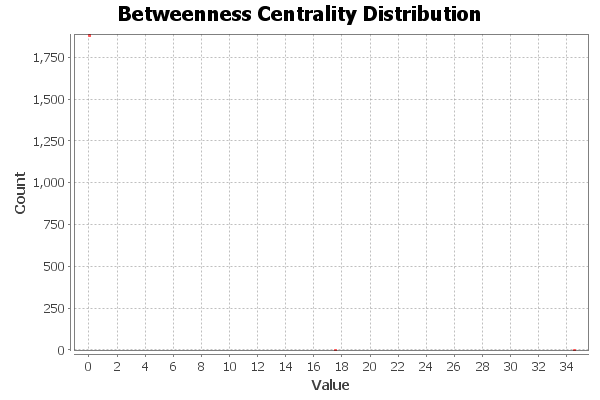
\includegraphics[width=\textwidth]{BetweennessCentralityDistribution.png}
                \caption{Betweenness Centrality Distribution}
               
        \end{subfigure}
        ~ %add desired spacing between images, e. g. ~, \quad, \qquad etc.
          %(or a blank line to force the subfigure onto a new line)
        
        \begin{subfigure}[b]{0.675\textwidth}
                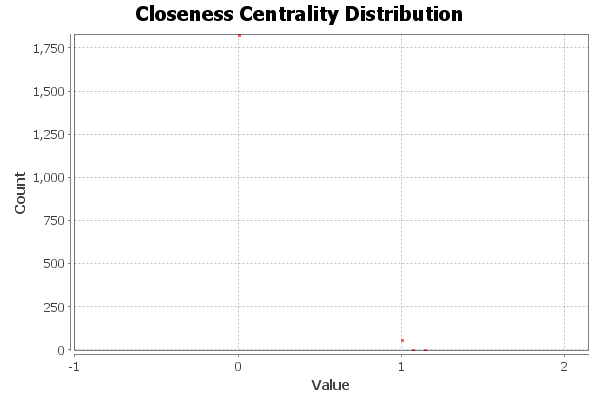
\includegraphics[width=\textwidth]{ClosenessCentralityDistribution.png}
                \caption{Closeness Centrality Distribution}
                
        \end{subfigure}%
        
         \begin{subfigure}[c]{0.675\textwidth}
                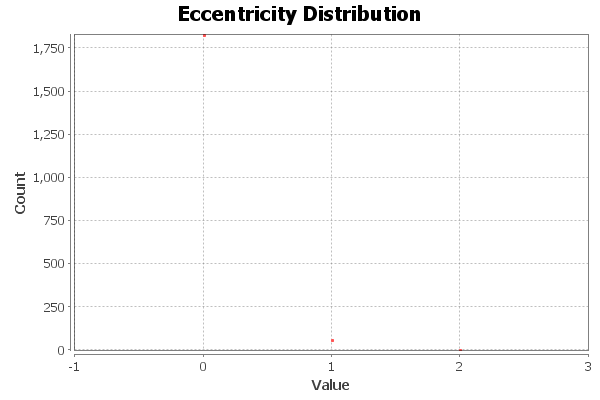
\includegraphics[width=\textwidth]{EccentricityDistribution.png}
                \caption{Eccentricity Distribution}
                
        \end{subfigure}%
        \caption{Network Diameter}
\end{figure}
\begin{figure}
\center
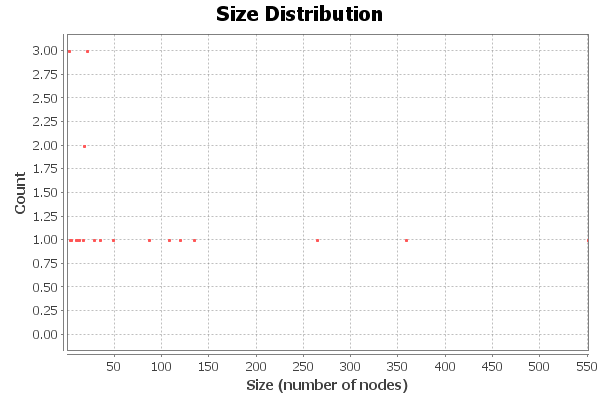
\includegraphics[width=\linewidth]{cc-size-distribution.png} 
\caption{Connected Components}
\end{figure}

\end{document}